\documentclass{extbook}[14pt]
\usepackage{multicol, enumerate, enumitem, hyperref, color, soul, setspace, parskip, fancyhdr, amssymb, amsthm, amsmath, bbm, latexsym, units, mathtools}
\everymath{\displaystyle}
\usepackage[headsep=0.5cm,headheight=0cm, left=1 in,right= 1 in,top= 1 in,bottom= 1 in]{geometry}
\usepackage{dashrule}  % Package to use the command below to create lines between items
\newcommand{\litem}[1]{\item #1

\rule{\textwidth}{0.4pt}}
\pagestyle{fancy}
\lhead{}
\chead{Answer Key for Makeup Progress Quiz -1 Version C}
\rhead{}
\lfoot{7547-2949}
\cfoot{}
\rfoot{Fall 2020}
\begin{document}
\textbf{This key should allow you to understand why you choose the option you did (beyond just getting a question right or wrong). \href{https://xronos.clas.ufl.edu/mac1105spring2020/courseDescriptionAndMisc/Exams/LearningFromResults}{More instructions on how to use this key can be found here}.}

\textbf{If you have a suggestion to make the keys better, \href{https://forms.gle/CZkbZmPbC9XALEE88}{please fill out the short survey here}.}

\textit{Note: This key is auto-generated and may contain issues and/or errors. The keys are reviewed after each exam to ensure grading is done accurately. If there are issues (like duplicate options), they are noted in the offline gradebook. The keys are a work-in-progress to give students as many resources to improve as possible.}

\rule{\textwidth}{0.4pt}

\begin{enumerate}\litem{
Determine the appropriate model for the graph of points below.

\begin{center}
    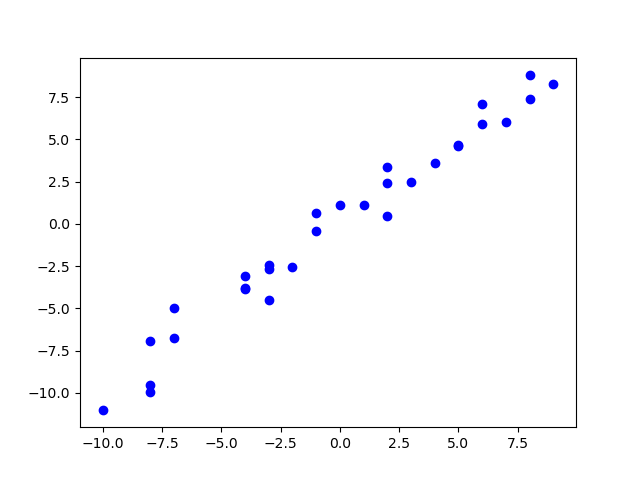
\includegraphics[width=0.5\textwidth]{../Figures/identifyModelGraph11C.png}
\end{center}




The solution is \( \text{Linear model} \), which is option B.\begin{enumerate}[label=\Alph*.]
\item \( \text{Exponential model} \)

For this to be the correct option, we want an extremely slow change early, then a rapid change later.
\item \( \text{Linear model} \)

For this to be the correct option, we need to see a mostly straight line of points.
\item \( \text{Logarithmic model} \)

For this to be the correct option, we want a rapid change early, then an extremely slow change later.
\item \( \text{Non-linear Power model} \)

For this to be the correct option, we need to see a polynomial or rational shape.
\item \( \text{None of the above} \)

For this to be the correct option, we want to see no pattern in the points.
\end{enumerate}

\textbf{General Comment:} This question is testing if you can associate the models with their graphical representation. If you are having trouble, go back to the corresponding Core module to learn about the specific function you are having trouble recognizing.
}
\litem{
The temperature of an object, $T$, in a different surrounding temperature $T_s$ will behave according to the formula $T(t) = Ae^{kt} + T_s$, where $t$ is minutes, $A$ is a constant, and k is a constant. Use this formula and the situation below to construct a model that describes the uranium's temperature, $T$, based on the amount of time t (in minutes) that have passed. Choose the correct constant $k$ from the options below.

\begin{center}
    \textit{ Uranium is taken out of the reactor with a temperature of $100^{\circ}$ C and is placed into a $11^{\circ}$ C bath to cool. After 14 minutes, the uranium has cooled to $34^{\circ}$ C. }
\end{center}


The solution is \( k = -0.09665 \), which is option C.\begin{enumerate}[label=\Alph*.]
\item \( k = -0.10498 \)

This uses $A$ as the initial temperature and solves for $k$ incorrectly.
\item \( k = -0.04081 \)

This uses $A$ correctly but solves for $k$ incorrectly.
\item \( k = -0.09665 \)

* This is the correct option.
\item \( k = -0.03996 \)

This uses $A$ as the initial temperature and solves for $k$ correctly.
\item \( \text{None of the above} \)

If you chose this, please contact the coordinator to discuss why you believe none of the other answers are correct.
\end{enumerate}

\textbf{General Comment:} The initial temperature is when $t = 0$. Unlike power models, that means $A$ is not the initial temperature!
}
\litem{
Determine the appropriate model for the graph of points below.

\begin{center}
    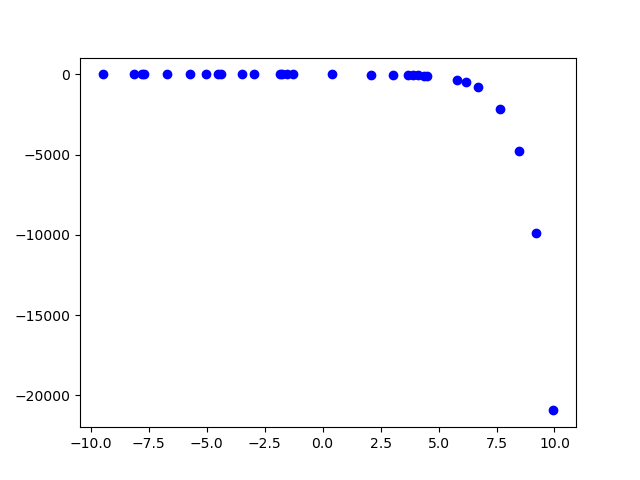
\includegraphics[width=0.5\textwidth]{../Figures/identifyModelGraph11CopyC.png}
\end{center}




The solution is \( \text{Exponential model} \), which is option B.\begin{enumerate}[label=\Alph*.]
\item \( \text{Logarithmic model} \)

For this to be the correct option, we want a rapid change early, then an extremely slow change later.
\item \( \text{Exponential model} \)

For this to be the correct option, we want an extremely slow change early, then a rapid change later.
\item \( \text{Linear model} \)

For this to be the correct option, we need to see a mostly straight line of points.
\item \( \text{Non-linear Power model} \)

For this to be the correct option, we need to see a polynomial or rational shape.
\item \( \text{None of the above} \)

For this to be the correct option, we want to see no pattern in the points.
\end{enumerate}

\textbf{General Comment:} This question is testing if you can associate the models with their graphical representation. If you are having trouble, go back to the corresponding Core module to learn about the specific function you are having trouble recognizing.
}
\litem{
Using the scenario below, model the situation using an exponential function and a base of $\frac{1}{2}$. Then, solve for the half-life of the element, rounding to the nearest day.

\begin{center}
    \textit{ The half-life of an element is the amount of time it takes for the element to decay to half of its initial starting amount. There is initially 947 grams of element $X$ and after 10 years there is 118 grams remaining. }
\end{center}


The solution is \( \text{About } 1095 \text{ days} \), which is option C.\begin{enumerate}[label=\Alph*.]
\item \( \text{About } 1460 \text{ days} \)

This uses the correct model but a base of $e$ rather than $\frac{1}{2}$.
\item \( \text{About } 365 \text{ days} \)

This models half-life as a linear function.
\item \( \text{About } 1095 \text{ days} \)

* This is the correct option.
\item \( \text{About } 4380 \text{ days} \)

This uses the correct model but solves for the exponential constant incorrectly.
\item \( \text{None of the above} \)

Please contact the coordinator if you believe all the options above are incorrect.
\end{enumerate}

\textbf{General Comment:} The model should be $A(t) = A_0 (\frac{1}{2})^{kt}$, where $A(t)$ is the amount after $t$ years, $A_0$ is the initial amount, and $k$ is decay constant. To find the half-life, you need to solve for $k$ by using the amount after $x$ years, then solve for the time $t$ when $A = \frac{A_0}{2}$. Your answer would be in years, so convert to days.
}
\litem{
The temperature of an object, $T$, in a different surrounding temperature $T_s$ will behave according to the formula $T(t) = Ae^{kt} + T_s$, where $t$ is minutes, $A$ is a constant, and k is a constant. Use this formula and the situation below to construct a model that describes the uranium's temperature, $T$, based on the amount of time t (in minutes) that have passed. Choose the correct constant $k$ from the options below.

\begin{center}
    \textit{ Uranium is taken out of the reactor with a temperature of $140^{\circ}$ C and is placed into a $18^{\circ}$ C bath to cool. After 13 minutes, the uranium has cooled to $81^{\circ}$ C. }
\end{center}


The solution is \( k = -0.05084 \), which is option A.\begin{enumerate}[label=\Alph*.]
\item \( k = -0.05084 \)

* This is the correct option.
\item \( k = -0.06142 \)

This uses $A$ as the initial temperature and solves for $k$ incorrectly.
\item \( k = -0.05364 \)

This uses $A$ as the initial temperature and solves for $k$ correctly.
\item \( k = -0.05491 \)

This uses $A$ correctly but solves for $k$ incorrectly.
\item \( \text{None of the above} \)

If you chose this, please contact the coordinator to discuss why you believe none of the other answers are correct.
\end{enumerate}

\textbf{General Comment:} The initial temperature is when $t = 0$. Unlike power models, that means $A$ is not the initial temperature!
}
\litem{
Using the scenario below, model the population of bacteria $\alpha$ in terms of the number of minutes, $t$ that pass. Then, choose the correct approximate \textit{(rounded to the nearest minute)} replication rate of bacteria-$\alpha$.

\begin{center}
    \textit{ A newly discovered bacteria, $\alpha$, is being examined in a lab. The lab started with a petri dish of 4 bacteria-$\alpha$. After 2 hours, the petri dish has 139 bacteria-$\alpha$. Based on similar bacteria, the lab believes bacteria-$\alpha$ doubles after some undetermined number of minutes. }
\end{center}


The solution is \( \text{None of the above} \), which is option E.\begin{enumerate}[label=\Alph*.]
\item \( \text{About } 362 \text{ minutes} \)

This uses the wrong base, does not solve for the constant correctly, AND converted incorrectly.
\item \( \text{About } 222 \text{ minutes} \)

This uses the wrong base and solves for the constant correctly but converted incorrectly.
\item \( \text{About } 37 \text{ minutes} \)

This uses the wrong base.
\item \( \text{About } 60 \text{ minutes} \)

This uses the wrong base and does not solve for the constant correctly.
\item \( \text{None of the above} \)

* This is the correct option as all other options used the wrong base in their model.
\end{enumerate}

\textbf{General Comment:} Your model should be $P(t) = P_0(b)^{kt}$, where $P(t)$ is the population at some time $t$, $P_0$ is the initial population, and $k$ is the replication rate. Be sure you convert the hours into minutes!
}
\litem{
A town has an initial population of 90000. The town's population for the next 10 years is provided below. Which type of function would be most appropriate to model the town's population?



\begin{tabular}{c|c|c|c|c|c|c|c|c|c}
\textbf{Year} & 1 & 2 & 3 & 4 & 5 & 6 & 7 & 8 & 9 \tabularnewline
\hline
\textbf{Pop.} & 90020 & 90040 & 90060 & 90080 & 90100 & 90120 & 90140 & 90160 & 90180
\end{tabular} 

The solution is \( \text{Linear} \), which is option C.\begin{enumerate}[label=\Alph*.]
\item \( \text{Logarithmic} \)

This suggests the slowest of growths that we know.
\item \( \text{Non-Linear Power} \)

This suggests a growth faster than constant but slower than exponential.
\item \( \text{Linear} \)

This suggests a constant growth. You would be able to add or subtract the same amount year-to-year if this is the correct answer.
\item \( \text{Exponential} \)

This suggests the fastest of growths that we know.
\item \( \text{None of the above} \)

Please contact the coordinator to discuss why you believe none of the options model the population.
\end{enumerate}

\textbf{General Comment:} We are trying to compare the growth rate of the population. Growth rates can be characterized from slowest to fastest as: logarithmic, indirect, linear, direct, exponential. The best way to approach this is to first compare it to linear (is it linear, faster than linear, or slower than linear)? If faster, is it as fast as exponential? If slower, is it as slow as logarithmic?
}
\litem{
A town has an initial population of 50000. The town's population for the next 10 years is provided below. Which type of function would be most appropriate to model the town's population?



\begin{tabular}{c|c|c|c|c|c|c|c|c|c}
\textbf{Year} & 1 & 2 & 3 & 4 & 5 & 6 & 7 & 8 & 9 \tabularnewline
\hline
\textbf{Pop.} & 50000 & 50020 & 50032 & 50041 & 50048 & 50053 & 50058 & 50062 & 50065
\end{tabular} 

The solution is \( \text{Logarithmic} \), which is option D.\begin{enumerate}[label=\Alph*.]
\item \( \text{Linear} \)

This suggests a constant growth. You would be able to add or subtract the same amount year-to-year if this is the correct answer.
\item \( \text{Exponential} \)

This suggests the fastest of growths that we know.
\item \( \text{Non-Linear Power} \)

This suggests a growth faster than constant but slower than exponential.
\item \( \text{Logarithmic} \)

This suggests the slowest of growths that we know.
\item \( \text{None of the above} \)

Please contact the coordinator to discuss why you believe none of the options model the population.
\end{enumerate}

\textbf{General Comment:} We are trying to compare the growth rate of the population. Growth rates can be characterized from slowest to fastest as: logarithmic, indirect, linear, direct, exponential. The best way to approach this is to first compare it to linear (is it linear, faster than linear, or slower than linear)? If faster, is it as fast as exponential? If slower, is it as slow as logarithmic?
}
\litem{
Using the scenario below, model the situation using an exponential function and a base of $\frac{1}{2}$. Then, solve for the half-life of the element, rounding to the nearest day.

\begin{center}
    \textit{ The half-life of an element is the amount of time it takes for the element to decay to half of its initial starting amount. There is initially 787 grams of element $X$ and after 12 years there is 87 grams remaining. }
\end{center}


The solution is \( \text{About } 1095 \text{ days} \), which is option D.\begin{enumerate}[label=\Alph*.]
\item \( \text{About } 1825 \text{ days} \)

This uses the correct model but a base of $e$ rather than $\frac{1}{2}$.
\item \( \text{About } 365 \text{ days} \)

This models half-life as a linear function.
\item \( \text{About } 5840 \text{ days} \)

This uses the correct model but solves for the exponential constant incorrectly.
\item \( \text{About } 1095 \text{ days} \)

* This is the correct option.
\item \( \text{None of the above} \)

Please contact the coordinator if you believe all the options above are incorrect.
\end{enumerate}

\textbf{General Comment:} The model should be $A(t) = A_0 (\frac{1}{2})^{kt}$, where $A(t)$ is the amount after $t$ years, $A_0$ is the initial amount, and $k$ is decay constant. To find the half-life, you need to solve for $k$ by using the amount after $x$ years, then solve for the time $t$ when $A = \frac{A_0}{2}$. Your answer would be in years, so convert to days.
}
\litem{
Using the scenario below, model the population of bacteria $\alpha$ in terms of the number of minutes, $t$ that pass. Then, choose the correct approximate \textit{(rounded to the nearest minute)} replication rate of bacteria-$\alpha$.

\begin{center}
    \textit{ A newly discovered bacteria, $\alpha$, is being examined in a lab. The lab started with a petri dish of 4 bacteria-$\alpha$. After 1 hours, the petri dish has 70 bacteria-$\alpha$. Based on similar bacteria, the lab believes bacteria-$\alpha$ quadruples after some undetermined number of minutes. }
\end{center}


The solution is \( \text{About } 29 \text{ minutes} \), which is option C.\begin{enumerate}[label=\Alph*.]
\item \( \text{About } 39 \text{ minutes} \)

This does not solve for the constant correctly.
\item \( \text{About } 174 \text{ minutes} \)

This solves for the constant correctly but converted incorrectly.
\item \( \text{About } 29 \text{ minutes} \)

* This is the correct option.
\item \( \text{About } 234 \text{ minutes} \)

This does not solve for the constant correctly AND converted incorrectly.
\item \( \text{None of the above} \)

Please contact the coordinator to discuss why you believe none of the answers above are correct.
\end{enumerate}

\textbf{General Comment:} Your model should be $P(t) = P_0(b)^{kt}$, where $P(t)$ is the population at some time $t$, $P_0$ is the initial population, and $k$ is the replication rate. Be sure you convert the hours into minutes!
}
\end{enumerate}

\end{document}